\documentclass[../summary.tex]{subfiles}

\begin{document}
	
	\section{Economics for sustainability}
	
	\subsection{Study guide}
	
	The study guide for chapter 10 of the MOOC was a complete mess. That is why, even though this part of the summary is still based on the study guide, there won't be an overview of it in this summary.
	\\\\
	Typical questions are:
	\begin{itemize}
		\item Definitions, terminology: be able to explain the definition, give examples
		\item Graphs: be able to explain and interpret the graphs
		\item Principles: be able to explain, give examples
	\end{itemize}
	
	\subsection{Gross Domestic Product}
	
	The Gross Domestic Product or GDP is a measure of total production that is used to reflect the economic health of a country or region and has strongly increased since the end of the 19th century. Figure \ref{fig:GDP} shows this exponential growth.
		
	\begin{figure}[htbp]
		\centering
		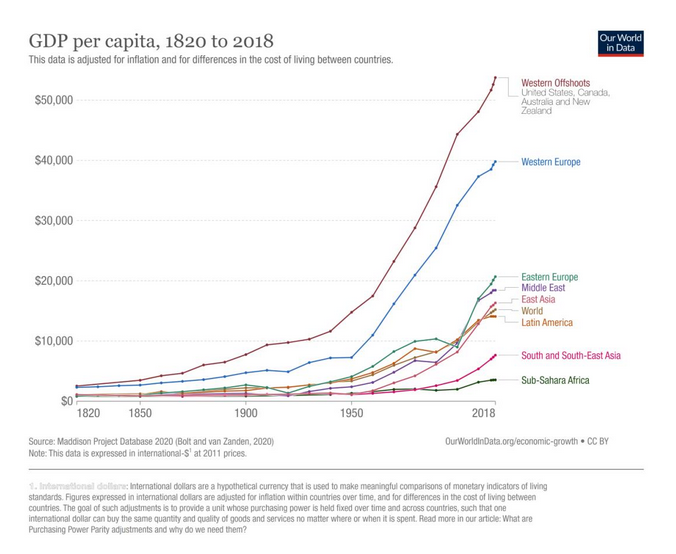
\includegraphics[width=1\linewidth]{images/10-GDP-increase.png}
		\caption{Increase in GDP since 19th century}
		\label{fig:GDP}
	\end{figure}
	
	\newpage
	This increase in GDP went together with a lot of other positive phenomena, such as an increase in life expectancy, an increase in literacy, a decrease in hunger, and so on. However, at the same time, we also saw a rise in environmental pressures, such as greenhouse gas emissions, global warming, plastic pollution, declining biodiversity, and many more. 
	\\\\
	Economic growth is the annual percentage change of real GDP. Real GDP means it's GDP measured in monetary terms but it's corrected for inflation and price changes.
	
	
\end{document}